\documentclass{article}
\usepackage [spanish]{babel}
\usepackage{graphicx} % Required for inserting images

\title{Teoría del universo}
\author{Alexa Dorantes Torres}
\date{27 de septiembre 2026}

\begin{document}

\maketitle

\section{Mi propia teoría}
\maketitle
En mi percepción el universo se creo por un error, no necesariamente por una explosión o porque apareció de la nada en la "nada", mi explicación lógica es que había un átomo súper pequeño que vagaba por una cosa distinta y más grande que el universo, luego comenzó a evolucionar y a ser más grande de poco en poco hasta que hubo un punto en el que creó más que un espacio vació, pudo haber iniciado con las estrellas y cuando una moría se dispersaba; estas pequeás cositas que generaba se hicieron planetas, lunas, más extrellas, nebulosas, entre otros elementos de lo que conocemos como "nuestro universo" pero de poco en poco se distribuyó hasta ser a su manera.
Una cita que reflejaría mi punto de vista sería la siguiente:

\begin{center}
\textbf{\textit{"Debido a la existencia de una ley como la de la gravedad, el universo puede y se creará a sí mismo de la nada. La creación espontánea es la razón por la que existe algo en lugar de nada, por la que existe el universo, por la que existimos nosotros."}} \\
\end{center}

\begin{center} 
\textbf{Stephen Hawking, en su libro El gran diseño (2010).}
\end{center}


En otro punto entra que el universo puede llegar a ser un bucle infinito de existencia en si mismo; sería tipo que no dimensiona bien su tamaño, y aunque una cosa puede ser muy pequeña entra algo más grande; yo lo asimilo mucho con que se ve relativamente lo mismo si observarás la galaxia con un telescopio a si mirarás una molecula con un microscopio, los componentes son lo mismos porque al final se compone de lo mismo en distintas cantidades pero abriendo un poco más la mente, ¿qué nos diría que si oberservas desde el microscopio no estámos viendo planetas y formas de vida que por simple resolución no alcanzamos a asimilar?.\\
Yo por ejemplo proponía que se vería como una dona en la cual evidentemente nada se puede salir pero da como vueltas entre si, sin embargo hace unos meses leí algo sobre unos científicos, específicamente el mecanismo de Higgs y la ruptura espontánea de la simetría.


\begin{center}
\textbf{\textit{"Es de interés notar que el estado de vacío ordinario (el estado de menor energía) se vuelve inestable... Como consecuencia, el campo escalar adquiere un valor esperado en el vacío diferente de cero. Esto provoca que ciertos campos que antes no tenían masa, la adquieran de forma automática gracias a esta interacción".}}
\end{center}

\begin{center} 
\textbf{Higgs, P. W. (1964). Broken Symmetries and the Masses of Gauge Bosons. Physical Review Letters, 13(16), 508–509. doi.org.}
\end{center}


Años despúes de todos los conocimientos que brindó Higgs, científicos quisieron graficar tridimensionalmente cómo se vería graficada una ecuación matemática pura, por lo tanto el "sombrero mexicano" es la representación visual de una fórmula.


\begin{figure}[h]
    \centering
    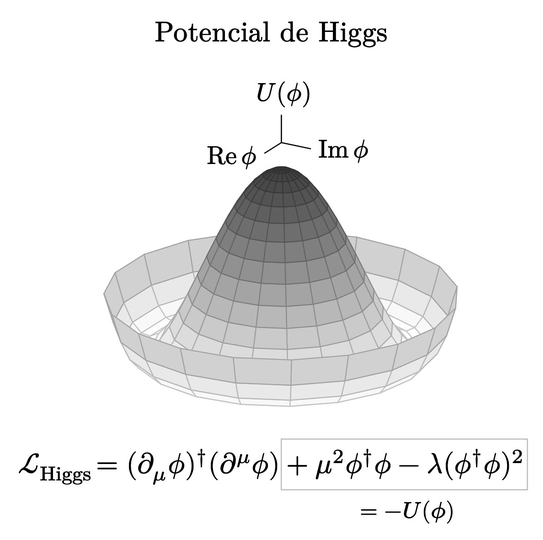
\includegraphics[width=0.5\linewidth]{Captura desde 2026-09-27 20-22-34.png}
    \caption{Representación grafica del sombrero mexicano (Potencial de Higgs).}
    \label{fig:placeholder}
\end{figure}

\section{¿Cómo podría ser la construcción del universo?}
Yo siento que el universo aparte de que se creó con un propósito, se creó con un orden y una razón de ser, pero mi representación de universo no sería similar a la de todos los demás, en mi cabeza tiene una similitud muy grande con por ejemplo como ya he dicho los átomos, las moléculas y así entonces pondré en orden todos y buscaré que sea lo más comprensible para que se logré entender.

\textbf{Orden del universo en pares.}

\begin{enumerate}
    \item Los humanos son los átomos que conforman el universo.
    \item Los planetas son las moléculas que conforman el universo.
    \item Los distintos sistemas solares son los órganos del universo.
    \item Las redes cósmicas son las venas del universo.
    \item Las distintas galaxias dividen partes de un cuerpo por así decirlo, como los nervios
    \item Parte final, el cosmos.
\end{enumerate}

Mi punto con esto es que quién nos dice que no podemos ser parte de un ser más grande que nosotros y nosotros lo conformamos así como hay cosas que nos conforman a nosotros, que tal vez nuestra parte de un cuerpo es el cerebro y por ende la mente de ese ser.\\
Es complicado plantearlo, pero tal vez por eso mismo no podemos ver más allá de un alcance mínimo del universo, porque estamos retenidos dentro de algo; que por eso las galaxias y lo que las conforman se muevem.\\
Tal vez la complejidad en la creación del universo es la "simplesa" del proceso que tienen los humanos luego de ser nada dentro del vientre de una mujer y términar existiendo como un bebé con todos los tipos de componentes que ya antes mencioné.

\maketitle
\end{document}
